%!TEX TS-program = xelatex
%!TEX encoding = UTF-8 Unicode

\documentclass[11pt]{extarticle}
% extarticle is like article but can handle 8pt, 9pt, 10pt, 11pt, 12pt, 14pt, 17pt, and 20pt text

\def \ititle {Joint Action \& the Emergence of Mindreading}
\def \isubtitle {Lecture 2: Minimal Theory of Mind}
\def \iauthor {Stephen A. Butterfill and Ian Apperly}
\def \iemail{s.butterfill@warwick.ac.uk}
\date{}

\input{$HOME/Documents/submissions/preamble_steve_handout}


%itemize bullet should be dash
\renewcommand{\labelitemi}{$-$}

\begin{document}

\begin{multicols}{3}

\setlength\footnotesep{1em}

\bibpunct{}{}{,}{s}{}{,}  %use superscript TICS style bib

\bibliographystyle{newapa} %apalike

%\maketitle
%\tableofcontents






\begin{center}
{\Large
Mindreading \& Joint Action: Philosophical Tools}

Lecture 2: What Are Mental States?


ButterfillS@ceu.hu
\end{center}

\section{Background}
'Naturalism in epistemology is merely the attempt to get clear enough about what we mean when we talk about knowledge and perception to be able to tell—in ways a biologist or an experimental psychologist would recognise as scientifically respectable—whether what we are saying is true.'\citep%[p.\ x]
{Dretske:2000ky}

`One thing missing, or rare, in this research with young children is a sense of how, if at all, they understand various psychological states as fitting together.'\citep{Wellman:2000cd}


\section{Sample Claims}
‘chimpanzees understand … intentions … perception and knowledge … Moreover, they understand how these psychological states work together to produce intentional action’\citep{Call:2008di} %(Call & Tomasello 2008:191)

‘from 7 months on ... humans automatically compute other’s beliefs and seem to hold them in mind as alternative representations of the environment.’\citep{kovacs_social_2010} %(Kovács et al 2010: 1834)

`an early [in human development] internal-state, yet interconnected, understanding of people gives way to a later mental–representational and still more interconnected understanding of mind'\citep{Wellman:2000cd} %p. 911

\section{What Is Knowledge?}
‘our fundamental conception of what it is to know that P is itself an explanatory conception […] we think of S’s knowledge that P as something that can properly be explained by reference to what S has perceived or remembered or proved or ...’\citep{Cassam:2007ri} %(Cassam 2007: 356)


\section{Mental States}
\begin{center}
  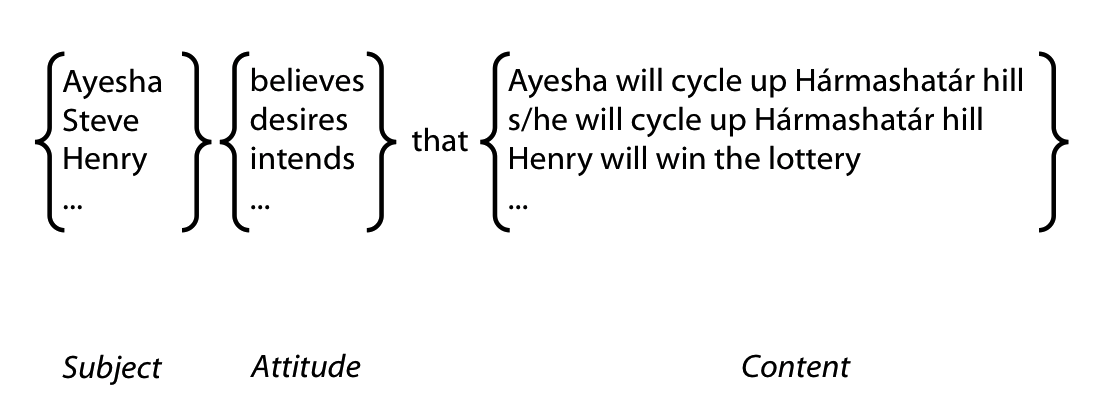
\includegraphics[width=0.3\textwidth]{fig4n.png}
\end{center}


\section{Propositions: how to mystify them}
‘Propositions ... are the sharable objects of the attitudes and the primary bearers of truth and falsity’\citep{McGrath:2012pro} (?!)

\section{Indexicals}
`If I see, reflected in a window, the image of a man whose pants appear to be on fire, my behaviour is sensitive to whether I think, ``His pants are on fire'', or ``My pants are on fire'', though the object of thought may be the same.'\citep{Kaplan:1990xa} %p.\ 42

\section{Maps or sentence-like objects?}
`what is inside our heads should be thought of as more like maps than sentences'\citep{Braddon-Mitchell:1996ce} %p.\ 163

\section{Defining belief: normativity}
‘For any p: One ought to believe that p only if p.

‘the holding of this norm is one of the defining features of the notion of belief [...]. The truth is what you ought to believe, whether or not you know how to go about it, and whether or not you know if you have attained it. That, in my view, is what makes it the state that it is.’\citep{boghossian:2003_normativity} %(Boghossian 2003: 37, 38-9)

`belief must be characterized, not just as the attitude having the motivational role, but rather as a truth directed species of that attitude: to believe a proposition is to regard it as true with the aim of thereby accepting a truth.'\citep{Velleman:2000fq} %(247)

‘Aside from our purposes in forming beliefs or in using beliefs as guides to action, there is nothing they should or shouldn’t be.  …  The only fault with fallacious reasoning, the only thing wrong or bad about mistaken judgements, is that, generally speaking, we don’t like them.  We do our best to avoid them.  They do not—most of the time at least—serve our purposes’\citep{Dretske:2000ky} %(Dretske 2000: 247-8)

‘The payments true ideas bring are the sole why of our duty to follow them.  Identical whys exist in the case of wealth and health.  Truth makes no other kind of claim and imposes no other kind of ought than health and wealth do.’\citep{James:1907ae} %(James 1907: 89)

\section{Defining intention: normativity}
`Rational intentions should be agglomerative. If at one and the same time I rationally intend to A and rationally intend to B then it should be both possible and rational for me, at the same time, to intend to A and B.'\citep{bratman_faces_1999} %(Bratman 1999: 220)
 

\section{Decision theory illustration}
 
\begin{center}
  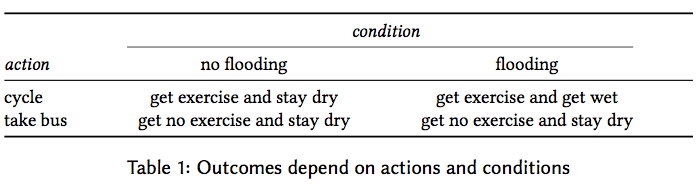
\includegraphics[width=0.3\textwidth]{table1.png}
\end{center}

\begin{center}
  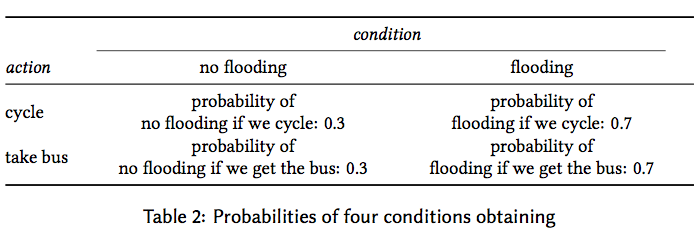
\includegraphics[width=0.3\textwidth]{table2.png}
\end{center}

\begin{center}
  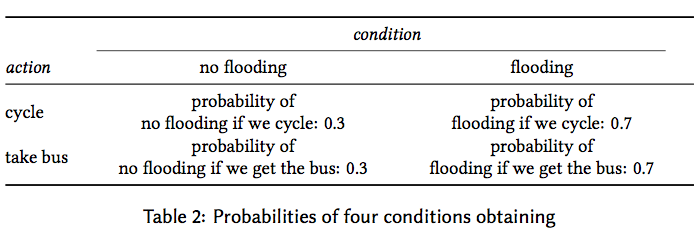
\includegraphics[width=0.3\textwidth]{table2.png}
\end{center}

\begin{center}
  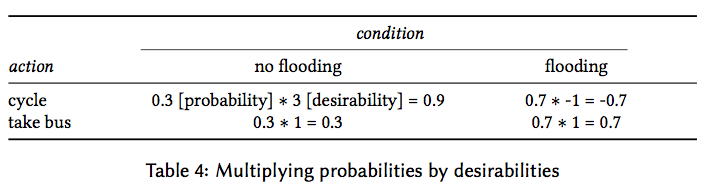
\includegraphics[width=0.3\textwidth]{table4.png}
\end{center}


\section{Ramsey's criterion}
`Suppose that A and B are consequences [outcomes] between which the agent is not indifferent, and that N is an ethically neutral condition [i.e.\ the agent is indifferent between N and not N]. 
%strictly:  p 46: A con- dition is ethically neutral in relation to a particular agent and a particular consequence if the agent is indifferent between having that consequence when the condition holds and when it fails.
Then N has probability 1/2 if and only if the agent is indifferent between the following two gambles:
	\\ \hspace*{10 mm} B if N, A if not 
	\\ \hspace*{10 mm} A if N, B if not'%
	\citep%[p.\ 47]
	{Jeffrey:1983oe}


\section{A missing aspect}
`modern philosophers ... have no theory of thought to speak of. I do think this is appalling; how can you seriously hope for a good account of belief if you have no account of belief fixation?'%
\citep%[p.\ 147]
{Fodor:1987rt}




\footnotesize 
\bibliography{$HOME/endnote/phd_biblio}

\end{multicols}

\end{document}